\documentclass[11pt, oneside]{article}   	% use "amsart" instead of "article" for AMSLaTeX format
\usepackage{geometry}                		% See geometry.pdf to learn the layout options. There are lots.
\geometry{letterpaper}    
\usepackage{float}               		% ... or a4paper or a5paper or ... 
%\geometry{landscape}                		% Activate for rotated page geometry
%\usepackage[parfill]{parskip}    		% Activate to begin paragraphs with an empty line rather than an indent
\usepackage{graphicx}				% Use pdf, png, jpg, or eps§ with pdflatex; use eps in DVI mode
\usepackage{tabularx}								% TeX will automatically convert eps --> pdf in pdflatex		
\usepackage{amssymb}
\usepackage{amsmath}

%SetFonts

%SetFonts


\title{Randomized Algorithms Analysis}
\author{Wilmer Uruchi Ticona}
%\date{}							% Activate to display a given date or no date

\begin{document}
\maketitle

\begin{abstract}
The following is an experiment of the running time of three algorithms to find the median of a vector. The first algorithm is Random QuickSort followed by a selection of the $[n/2]$ (position of the median) item in the vector. The second algorithm is Random QuickSelect aiming for the $[n/2]$ (position of the median) item in the vector. The third and last algorithm is RMedian, a randomized algorithm to find the median.
\end{abstract}
%\section{}
%\subsection{}

\section{The Experiment}

Three algorithms to find the median were implemented using python:
\begin{itemize}
\item Random $\textbf{QuickSort}$ $\hspace{5 mm}$ Expected complexity: $O(n \log n)$ $\hspace{5 mm}$ Worst case: $O(n^2)$

\item Random $\textbf{QuickSelect}$ $\hspace{5 mm}$ Expected complexity: $O(n)$ $\hspace{5 mm}$ Worst case: $O(n^2)$
\item $\textbf{RMedian}$ $\hspace{5 mm}$ Expected complexity: $O(n)$
\end{itemize}

The code also includes a data generation class that builds the sample data for the experiment. For this case 200 vectors were generated, each with 50001 random 3-digit integers. In order to expand the sample space of the experiment, the first 100 vectors were left as they were generated, distributed uniformly at random, the next 50 vectors were ordered in ascending order, and the last 50 vectors were ordered in descending order. As a result, the python program generated the file $data.txt$, where the vectors are stored in an easy-to-read array, where the vectors are distributed in the following way:

\begin{itemize}
\item $\textbf{0-99}$ (Vectors not ordered)
\item $\textbf{100-149}$ (Vectors in ascending order)
\item $\textbf{150-199}$ (Vectors in descending order)
\end{itemize}

Then, the vectors in the file are read by the $RandomTests$ class of the program. This class hosts in its methods the algorithms that are going to be run for the experiment. After reading the data, the class stores the data in a 2-dimensional array, and then performs the 3 algorithms for each of the 200 vectors. Code has been implemented to make sure that each algorithm receives the same input for each case. After all the experiments have been performed, the program stores the results in the file $resultsExperiment.txt$.

The results are stored in the form of data separated by commas that follows the structure:

\begin{table}[H]
\caption{Results Structure}
 \begin{tabularx}{\columnwidth}{|c|X|}
 \hline
  Column & Detail\\
  \hline \hline
  Array & Index of vector (array).\\
  timeQSort & Running time of algorithm in seconds.\\
  timeQSelect & Running time of algorithm in seconds.\\ 
  timeRMedian & Running time of algorithm in seconds.\\ 
  RMedianSuccess & Shows the result of RMedian (to identify when it fails).\\ 
 \hline
\end{tabularx}
\label{table: results structure}
\end{table}

After the experiment has been completed and the results have been generated, this file is imported into $RStudio$ to build the corresponding scatter plot and data summary table:

\begin{figure}[H]
\centering
  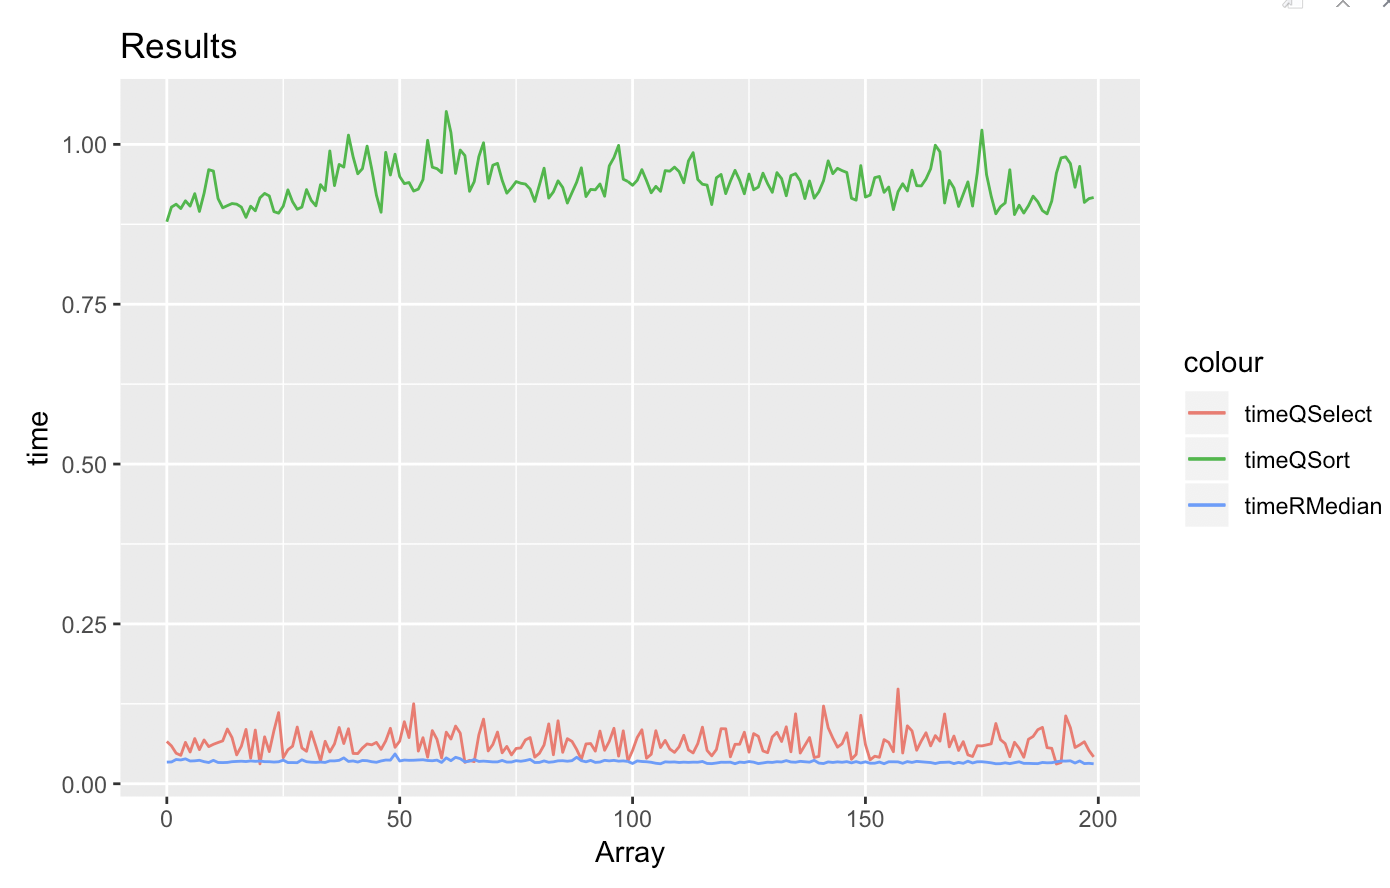
\includegraphics[scale=0.45]{plotexp.png}
  \caption{Plot of results}
  \label{fig:random1}
\end{figure}

\begin{figure}[H]
\centering
  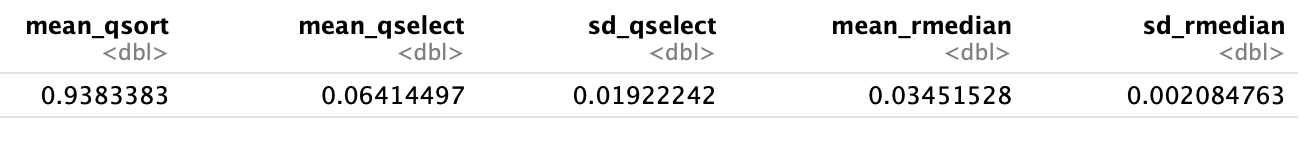
\includegraphics[scale=0.7]{sumexp.png}
  \caption{Summary of results}
  \label{fig:ransum1}
\end{figure}


\section{Which algorithm is faster?}

As we can see in the scatter plot of the result of the experiment, the mean running time of Random QuickSelect and RMedian are very close, and both are much lower than the mean running time of Random QuickSort. Between them, Random QuickSelect shows a higher standard deviation because, although of expected complexity $O(n)$, has a worst case scenario complexity of $O(n^2)$. By using the randomized version of this algorithm we are making the probability of hitting the worst case scenario very low, however, there are scenarios that will generate the variation found in the results. On the other hand, RMedian maintains a nearly linear running time, which is assured by the algorithm, and a mean running time of almost half of that of Random QuickSelect.

Although there is at least one case in which Random QuickSelect performed better than RMedian (in a vector that was already ordered in descending order), it is almost certain that RMedian will perform better in the vast majority of cases. In conclusion, $\textbf{RMedian}$ is the faster algorithm.

\section{Which algorithm is more reliable?}

We have concluded that RMedian is the faster algorithm. There is the fact that Random QuickSort and Random QuickSelect are always going to give a result, but in an expected running time higher than that of RMedian. However, RMedian does not always guarantee a result. There are three events so that if at least one of them happen, the result would be ``FAIL", indicating that the algorithm couldn't find the median. These events are:

$Event_1 : Y_1 = |{r \in R | r \leq m}| < \dfrac{1}{2}n^{3/4} - \sqrt{n}$\\
If this happens, then the median was not in the sample space.

$Event_2 : Y_2 = |{r \in R | r \geq m}| < \dfrac{1}{2}n^{3/4} - \sqrt{n}$\\
If this happens, then the median was not in the sample space.

$Event_3 : |C| > 4n^{3/4}$\\
The sample space is too big to guarantee linear time.\\

By Applying Chebyshev's inequality it is possible to bound the probability of $Event_1$:

$$Pr[Event_1] \leq \dfrac{1}{4}n^{-1/4}$$

We also know a bound for the probability of $Event_3$, that is, that the median was not in the sample space:

$$Pr[Event_3] \leq \dfrac{1}{2}n^{-1/4}$$

If $Event_3$ happens, then at least one of these two events happens:\\

$Event_{3,1} :$ at least $2n^{3/4}$ elements of $C$ are greater than the median.

$Event_{3,2} :$ at least $2n^{3/4}$ elements of $C$ are smaller than the median.\\

Again, applying Chebyshev's inequality we can find a bound for these events (they have the same bound because of symmetry).

$$Pr[Event_{3,2}] \leq \dfrac{1}{4}n^{-1/4}$$

So we have that:

$$Pr[Event_3] \leq Pr[Event_{3,1}] + Pr[Event_{3,2}] \leq \dfrac{1}{2}n^{-1/4}$$

Combining the bounds, we have that the probability that the algorithm outputs FAIL is bounded by:

$$Pr[Event_{1}] + Pr[Event_{2}] + Pr[Event_{3}] \leq n^{-1/4}$$

In the case of the experiments performed, that would be:

 $$Pr[FAIL] \leq 50001^{-1/4}$$
 
This bound is fairly high, but it is possible to build an iterative version of RMedian that guarantees a solution with a random running time. This version of the RMedian algorithm will have an expected linear running time.

In conclusion, in its current state (not iterative) we cannot say that RMedian is more reliable than Randomized QuickSelect or Random Pivot QuickSort, which always return a valid solution. So the option is between them, and in that case I think the faster one, $\textbf{Randomized QuickSelect}$ would satisfy most criteria to be considered the most reliable of the three.




\end{document}  